\chapter{Algorithmical Design}
  Even for a simple scenario like in figure \ref{fig:graphseen}, where we have a lot of possible links between the modules it is not obvious how to
  chose a low-interference network topology from this graph.
  A shortsighted solution may be trying to use every possible link, since this would decrease overall traveltimes for each packet and therefore
  reduncing network workload and possible interferences as a packet is not longer in the network than it needs to be. 
  The problem in doing so is the small number of channels we can assign to these links, even if we allow using multiple channels.
  Since we can only assign one channel to a module, trying to start small and assigning one channel to one module would then force us to also 
  assign the same channel to all connected modules in order to maintain connectivity as two modules can only communicate with each other if they use the same channel
  (See upper figure in \ref{fig:high_con_vs_low_con}). 
  
  \begin{figure}[h!]
    \centering
    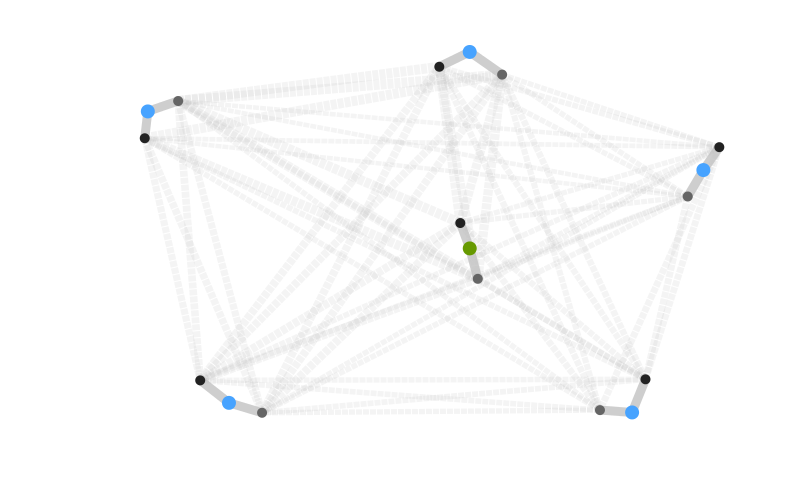
\includegraphics[width=0.8\columnwidth]{figures/graphseen.png}
    \caption{Network topology graph for a simple scenario with 6 accesspoints / 2 modules each. The green node indicates a connection to wired network.}
    \label{fig:graphseen}
  \end{figure}

  On the other hand if we only chose a very small subset of links in this graph (like a \ac{MST}), we might be able to 
  assign more channels, leading maybe up to no interference at all (See figure \ref{fig:high_con_vs_low_con}).
  As a drawback this could create bottlenecks, single points of failures and leading to packets staying longer in the 
  communication network since they can not take the shortest path. This is why we later need to add further links (survival paths).

  \begin{figure}[h!]
    \centering
    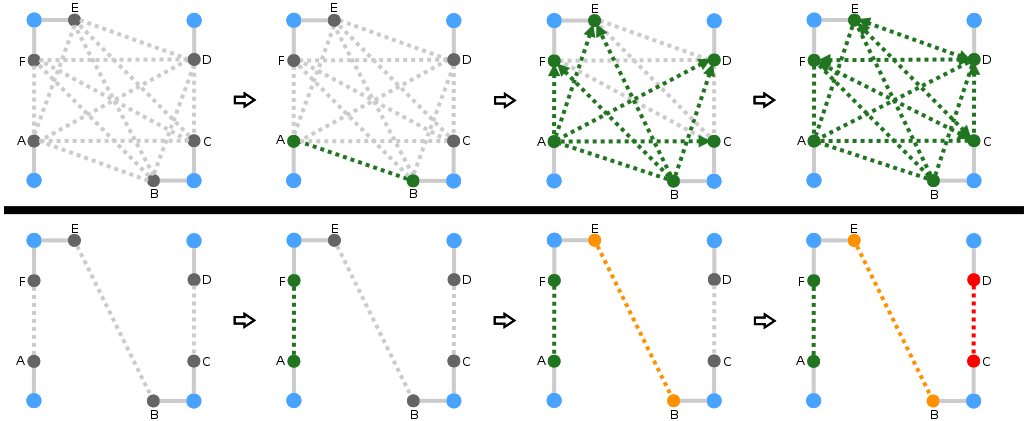
\includegraphics[width=1\columnwidth]{figures/high_con_vs_low_con.png}
    \caption{Coloring a highly connected network (upper) may result in fewer channels with high interference being used compared to 
      a reduced network topology (lower) where multiple interference-free channels can be used. Especially the dependent modules, which also have to receive the same channel
      in order to maintain connectivity are the reason for single channel usage here: Wanting to only color edge A,B you also have to assign the same channel to nodes C,D,E,F
      and therefore its edges.}
    \label{fig:high_con_vs_low_con}
  \end{figure}
  
  A consequence of the mono-channel setup in a dense topology line in figure \ref{fig:high_con_vs_low_con} is radical throughput performance loss as a transmission from
  A to B would prohibit any other communication due to the utiliazation of the same channel. Even if links (A,F), (E,B) and (D,C) would have a low link quality and packets
  can not travel directly to their destination a simultaneous transmission allows a higher throughput in the same time. Naturally only the second solution is favorable for a
  bigger scenario, because more APs would have to wait to put their data on the spectrum.
  Especially adding redundant links to a small subset of links in order to fulfill the reduced end-to-end link failure requirement is not straigh-forward as each newly
  added link increases overall throughput capacity, but at the same time may create co-channel interference or worse, decrease the number of overall assignable channels.
  
  \begin{figure}[h!]
    \centering
      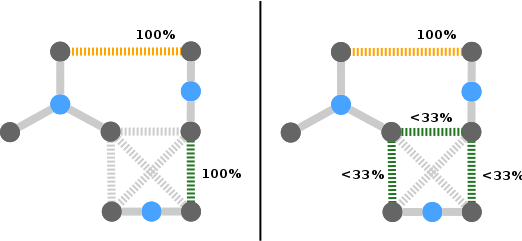
\includegraphics[width=\textwidth]{figures/lessismore}
      \caption{Additional links do not necessarily increase throughput performance rather on the contrary may decrease the number of non-interfering channels used (3 vs 2).
	Percentage depict link quality and therefore flow capacity.}
    \label{fig:lessismore}
  \end{figure}
  
  In the following two sections we will present an algorithm creating network topolgies, seeking to find the best compromise, by first creating the topology and then
  assigning channels on the resulting topology as basis.
 
  \section{Topology Creation}
    Creating the topology is also split into two parts.
    First, creating a \ac{MST}, respecting a certain provided formula, which scores edges depending on their expected throughput.
    Second, adding redundancies in form of backup or parallel links to the \ac{MST}. 
    To make it more vivid we added an example after the algorithmic description.

    \subsection{Minimal Spanning Tree Topology}
      In order to select the edges we want to use for creating connections between the APs, we use a derivation of the \ac{DJP}-algorithm \cite{prim}\cite{jarnik}.
      The reason we chose a \ac{MST} algorithm over other techniques like all-pairs shortest path is, that a \ac{MST} gives us the best essential edges in a graph. 
      We can then extend these essential set of edges with further redundant edges if we have or want to (survival paths). 
      Adding more than the essential edges immediately plays in favor of interference, which we want to avoid by all means and so have to do so carefully.
      
      From the set of all nodes which are connected by edges, we start by selecting an arbitray initial node and mark it as visited. 
      All edges from this set of visited nodes to unvisited nodes are called productive edges.
      We keep those productive edges in a list sorted by their scores. The score of an edge is determined by the following formula:
      
      \begin{equation} \label{eq:edgescore}
	ES=\frac{b}{(i + 1 )* (c + 1)}
      \end{equation}
      
      where \textit{ES} is the score of this edge, \textit{b} is the expected bandwidth, \textit{i} is the number of 
      interfering modules and \textit{c} is the connected count of the corresponding nodes. 
      Dividing \textit{b} by \textit{i} and \textit{c} describes how the theoretically available bandwidth would have to be shared among other interfering radios.
      This characteristic results in a lower \textit{ES} for edges where the assumed throughput is lower due to interference by other radios.
      The following three subsections will explain the formula in more detail.
      
      For each round we determine from this list the edge with the highest score. If two links have the same \textit{ES} and different SNRs, we pick the edge with
      the higher \ac{SNR} as this edge has to share its channel among fewer participants and therefore results in higher throughput with fewer interference to the network.
      As a last resort if there is also a tie in \ac{SNR} values, we pick one at random. We then mark the new node as visited and add also the new links to the list.
      Finally we have to update the scores for each affected link and continue with the next round until all nodes are marked visited.
      The outcome is a minimal spanning tree for this graph with a custom evaluation function.
      
\newpage
      
      \subsubsection{Interfering Modules}
	Since the channel assignment has not taken place yet, we do not know which modules are actually interfering with this link if we would use it.
	However we do know to which other modules this module already has connections to and since those have to use the same channel in order to communicate with each
	other, we can derive an estimate as lower bound for the number of interfering modules for this link (A, B) by counting the following modules:
	Total interfering modules is equal to the number of visited nodes which we can reach by one hop over a module-module connection from node A and B.
	Those modules definetly interfer with our current connection, since they:
	
	\begin{itemize}
	\item are in range with at least one node of this connection (one hop distance)
	
	\item have to use the same channel (communication over module-module link)
	
	\item do actually interfere, because we already decided to use this connection (visited node)
	\end{itemize}

	The value is incremented by one, because if this connection would be used, itself again acts as a source for interference and it nicely solves the division by zero
	problem. With an increasing count in interfering modules, the value of the link decreases and vice versa. This reflects perfectly the concept of a shared medium.

      \subsubsection{Expected Bandwidth}
	describes the expected available bandwidth we assume to get for this link depending on the \ac{SNR}.
	For a given \ac{SNR} we can estimate the maximal possible thoughput since effective bitrate and therefore throughput is amongst others dependent on the \ac{SNR}
	and modulation which is continuously adjusted by the network driver for the radio module during operation.\footnote{The rate adaptation algorithm 
	which is used in LANCOM devices is Minstrel \cite{minstrel}.} 
	The bandwidth was chosen as the numerator, since it is effectively shared by the radio modules within range.
	
	As we can take from figure \ref{fig:snr_tp}, a higher \ac{SNR}-value results in more bandwidth available to use and share and works in favor of this edge.
	Note that the mapping of \ac{SNR} to achievable throughput may have to be adjusted for different hardware / devices / drivers. 
	In general the behaviour will stay the same, as a higher \ac{SNR} will necessarily result in a better modulation, which also increases throughput.
	
	\begin{figure}[h!]
	  \centering
	  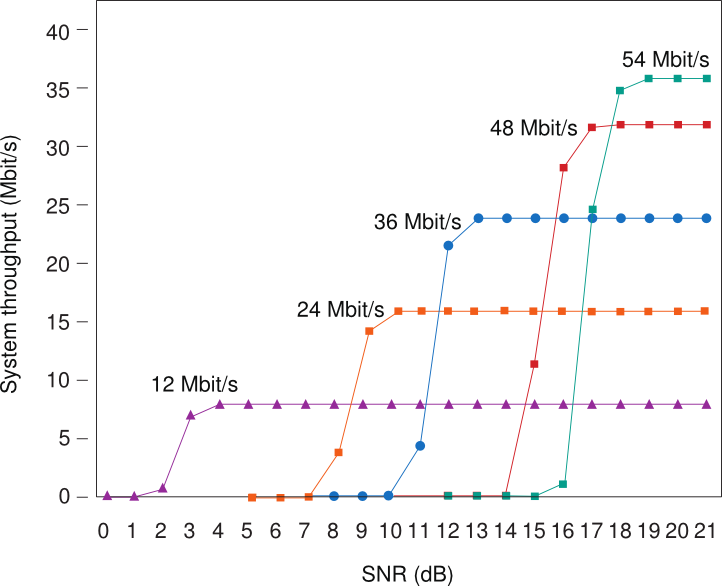
\includegraphics[width=0.6\columnwidth]{figures/snr_tp}
	  \caption{Expected throughput \ac{SNR}-values by \cite{expected_snr}. We assume to get the best possible throughput for a given \ac{SNR}, since 
	    modulation is automatically adapted by the APs with increasing \ac{SNR}.}
	  \label{fig:snr_tp}
	\end{figure}
	
	Another factor of influence would be the number of erroneous bytes that have been transmitted over this link. 
	This is hower not used for determining the expectet bandwidth as we do not know what those values are going to 
	look like before actually using this link to transmit data.
	
\newpage

      \subsubsection{Connected Count}
	Number of nodes we can reach from module A and module B by just using module-module edges (For example nodes A, B, C in figure \ref{fig:channel-list}). 
	A higher connected count diminishes the importance of this edge, since this value controls how many channels we can use later for the overall graph.
	If this value would not be taken into consideration for calculating the score, the algorithm would rather create long chains of connected modules. 
	Those links in this chain would admittedly have the best \ac{SNR} values, but since they have to share the same channel, 
	it would result in lowering the overall throughput. Granting this value a higher impact in the formula, like for example in 
	
	\begin{equation}
	  ES=\frac{b}{(i + 1)* (c + 1)^2}
	\end{equation}
	
	would have the effect of overemphasizing the module connectedness and lead to poor choices in links with respect to \ac{SNR} - 
	lowering overall throughput again. The simple, linear impact in the formula has shown to achieve the best tradeoff between those two extremes.
	
	\begin{figure}[h!]
	  \centering
	  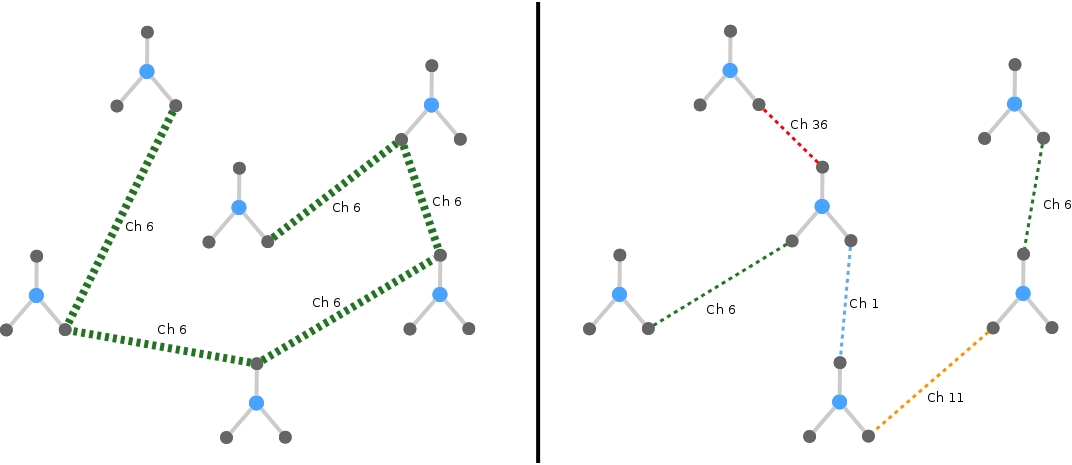
\includegraphics[width=1\columnwidth]{figures/formula_graphic}
	  \caption{Impact of the connected count on the formula. Resulting topology in case the connected count is underemphasized (left) leading
	    to long chains of possibly high quality links, but only one useable channel, which has to be shared among all modules.
	    Topology in case of an overemphasized connected count (right). As the algorithm avoids reutilizing already used modules,
	    links with low quality are preferred, leading a lot of exclusive channels with lower link quality. Thicker edges illustrate better link quality.}
	  \label{fig:formula_graphic}
	\end{figure}

\newpage
	
      \subsubsection{Example MST Creation}
	Let's take a look at a simplified example, where we assume \textit{b=SNR}. Also note that we immediately expand module-device edges to keep the example short.
	Normally the algorithm would also expand each of those edges step by step. However due to their maximum weight these have precedence over all other edges, 
	so that we merely skip a few tedious images.
	\begin{figure}[h!]
	  \centering
	  \begin{minipage}{0.5\textwidth}
	    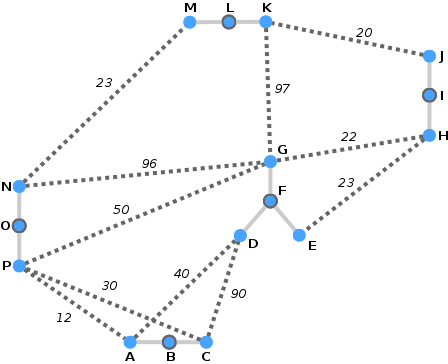
\includegraphics[width=\columnwidth]{figures/mst_calc_1}
	  \end{minipage}
	  \caption{Example input topology - Edge-weights representing the \ac{SNR}}
	  \label{fig:mst_calc_initial}
	\end{figure}
	
	Figure \ref{fig:mst_calc_initial} represents the underlying network topology with all possible links for a scenario with five APs where all APs are equipped with two
	radios except F, which has three.
	
	\begin{figure}[h!]
	  \centering
	  \begin{minipage}{7.4cm}
	    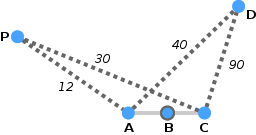
\includegraphics[width=4.5cm]{figures/mst_calc_2}
	  \end{minipage}
	  \begin{minipage}{4cm}
	    \begin{tabular}{c||c|c|c||c}
	      Edge & \textit{b} & \textit{i} & \textit{c} & \textit{ES}\\ \hline\hline
	      (A,D) & 40 & 0 & 0 & 40 \\ \hline
	      \textbf{(C,D)} & \textbf{90} & \textbf{0} & \textbf{0} & \textbf{90} \\ \hline
	      (A,P) & 12 & 0 & 0 & 12 \\ \hline
	      (C,D) & 30 & 0 & 0 & 30 \\ \hline
	    \end{tabular}
	  \end{minipage}
	  \caption{First round - Picking (C, D) with highest score}
	  \label{fig:mst_calc_2}
	\end{figure}
	
\newpage
	
	We start off by selecting a random node (B). Actually the first steps here would have been expanding the fake edges (B, A) and (B, C), 
	but as noted above we skip those. From this set of nodes we then consider all edges to newly, 
	up to now undiscovered nodes (listed in the right table in figure \ref{fig:mst_calc_2}).
	From this list of edges we calculate the \textit{ES} on each edge, which results in the selection of edge (C, D). 
	Note, from now on the values on the edges represent the \textit{ES} instead of \textit{b}.
	
	\begin{figure}[h!]
	  \centering
	  \begin{minipage}{7.5cm}
	    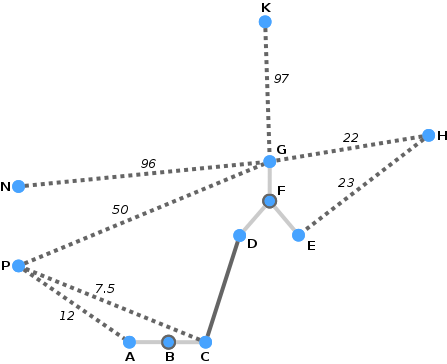
\includegraphics[width=7cm]{figures/mst_calc_3}
	  \end{minipage}
	  \begin{minipage}{4cm}
	    \begin{tabular}{c||c|c|c||c}
	      Edge & \textit{b} & \textit{i} & \textit{c} & \textit{ES}\\ \hline\hline
	      (A,P) & 12 & 0 & 0 & 12 \\ \hline
	      (C,P) & 30 & 1 & 1 & 7.5 \\ \hline
	      (G,P) & 50 & 0 & 0 & 50 \\ \hline
	      (G,N) & 96 & 0 & 0 & 96 \\ \hline
	      \textbf{(G,K)} & \textbf{97} & \textbf{0} & \textbf{0} & \textbf{97} \\ \hline
	      (G,H) & 22 & 0 & 0 & 22 \\ \hline
	      (E,H) & 23 & 0 & 0 & 23 \\ \hline
	    \end{tabular}
	  \end{minipage}
	\caption{Second round - Score for edge (C,P) decreased - Picking edge (G, K)}
	\label{fig:mst_calc_3}
      \end{figure}

      After the expansion of the fake edges for \ac{AP} F, we proceed by refreshing all the edgescores, 
      portraying edge (G, K) as the best edge (figure \ref{mst_calc_3}).
      Note how the score for edge (C, P) was decreased, since node C is already used for another edge.
      
      \begin{figure}[h!]
	\centering
	\begin{minipage}{7.5cm}
	  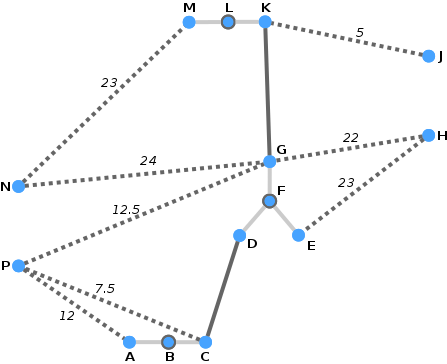
\includegraphics[width=7cm]{figures/mst_calc_4}
	\end{minipage}
	\begin{minipage}{4cm}
	  \begin{tabular}{c||c|c|c||c}
	    Edge & \textit{b} & \textit{i} & \textit{c} & \textit{ES}\\ \hline\hline
	    (A,P) & 12 & 0 & 0 & 12 \\ \hline
	    (C,P) & 30 & 1 & 1 & 7.5 \\ \hline
	    (G,P) & 50 & 1 & 1 & 12.5 \\ \hline
	    \textbf{(G,N)} & \textbf{96} & \textbf{1} & \textbf{1} & \textbf{24} \\ \hline
	    (G,H) & 22 & 1 & 1 & 5.5 \\ \hline
	    (E,H) & 23 & 0 & 0 & 23 \\ \hline
	    (K,J) & 20 & 1 & 1 & 5 \\ \hline
	    (M,N) & 23 & 0 & 0 & 23 \\ \hline
	  \end{tabular}
	\end{minipage}
	\caption{Third round - Best edge is (G,N).}
	\label{fig:mst_calc_4}
      \end{figure}
      
      All edges connected to G have been recalculated as G was used in the last step. Edge (G, N) is nevertheless the edge which promises accoding to 
      the formula the most throughput, even more than the up to now unused edge (E, H).
      
      \begin{figure}[h!]
	\centering
	\begin{minipage}{7.5cm}
	  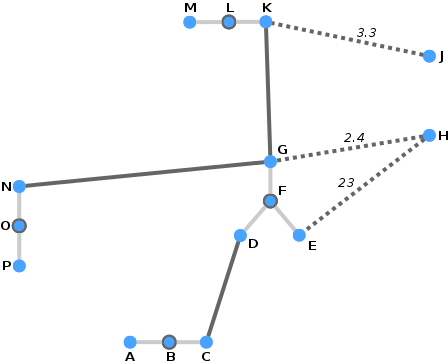
\includegraphics[width=7cm]{figures/mst_calc_5}
	\end{minipage}
	\begin{minipage}{4cm}
	  \begin{tabular}{c||c|c|c||c}
	    Edge & \textit{b} & \textit{i} & \textit{c} & \textit{ES}\\ \hline\hline
	    \textbf{(E,H)} & \textbf{23} & \textbf{0} & \textbf{0} & \textbf{23} \\ \hline
	    (G,H) & 22 & 2 & 2 & 2.4 \\ \hline
	    (K,J) & 20 & 1 & 2 & 3.3 \\ \hline
	  \end{tabular}
	\end{minipage}
	\caption{Fourth and final round - Best edge to connect the last nodes is (E,H)}
	\label{fig:mst_calc_5}
      \end{figure}
      
      Edgescores of the remaining links rapidly decrease as using these would definetly cause interference.
      This is the first step the connected count \textit{c} has a greater impact in calculating the \textit{ES} as the path N, G, K has length two.
      Using edge (G, H) would increase this distance to three, which would be unfavourable for the coloring process (all edges connected to G would have to use the same channel).
      Luckily we can utilize (E, H) which does not necessarily interfere with other links (it may interfere after the coloring process, if not enough colors are available).
      
      \begin{figure}[h!]
	\centering
	\begin{minipage}{7.5cm}
	  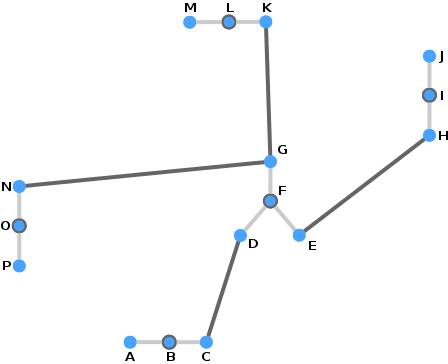
\includegraphics[width=7cm]{figures/mst_calc_6}
	\end{minipage}
	\begin{minipage}{4cm}
	  \hspace{4cm}
	\end{minipage}
	\caption{Resulting MST}
	\label{fig:mst_calc_6}
      \end{figure}  
     \newpage
      
    \subsection{Survival Paths}
      A spanning tree is very susceptible to graph partition by just removing or failing one link so we have to add redundancies in form of supplementary connections.
      However those redundant connections have to be carefully chosen in order not to negatively impact the successive channel assignment and therefore to push interference.
      Note that this is an optional feature, since for some usecases a spanning tree topology is enough or a topology with redundand links is not easily implemented
      with the existing code or hardware.  
      
      We accomplish this by iterating over all the edges of the spanning tree and simulate each connection failing. 
      We then check if there still exists a path from node A to node B of this failing connection. 
      Only if this failing connection cuts the graph in half and there is no path to the other side,
      we start looking for a backup route in the following fashion:
      First we separate the graph into two groups: Group A with all nodes and links reachable from node A and group B with the same for node B.
      We create a list with unused edges which connect the two groups and calculate the scores on them and pick again the edge with the highest score.
      This edge is the best edge to reconnect the two parts (according to the formula) and is called the survival edge for this failing scenario.
      Nevertheless we have to be aware that it might not be feasible to reconnect those parts if the underlying structure does not permit it.
      For example the link between nodes \(E\) and \(F\) in \ref{fig:survival_algo} might be the only connection possible and failing it would cause network disruption.
      But if this link fails there is nothing we can do. The result is a robust network topology, 
      which despite the added interfering links still yields a high overall throughput with redundant paths.

      The survival path attribute for a graph can also be expressed in the following formal way:
      \begin{quote}
	For each edge (a, b) of the calculated spanning tree graph G', find a path from a to b without traversing (a, b), 
	in a way that the sum of the Edgescores of the path is maximal.
      \end{quote}
      Description:
      $$\textit{G}=(\textit{V},\textit{E}) \quad
	\forall \textit{edge}_\textit{a,b} \exists \textit{path}_\textit{a,b} | \textit{edge}_\textit{a,b} \notin \textit{path}_\textit{a,b} \quad
	\textit{a,b} \in \textit{V}, \textit{edge}_\textit{a,b} \in \textit{E}$$
	Finding the optimal edge:
	$$\textit{max}(\textit{edgescore}(\textit{path}_\textit{a,b})) |
	\textit{edgescore}(\textit{path}_\textit{a,b})) = \sum_{\substack{e \in \textit{path}_\textit{a,b}}} \textit{edgescore}(e)$$
	
    Using survival path actively and additionally to the \ac{MST} links, instead of a fallback, 
    would require a shortest path routing that deals with circles in the graph.
   
    \begin{figure}[h!]
      \centering
      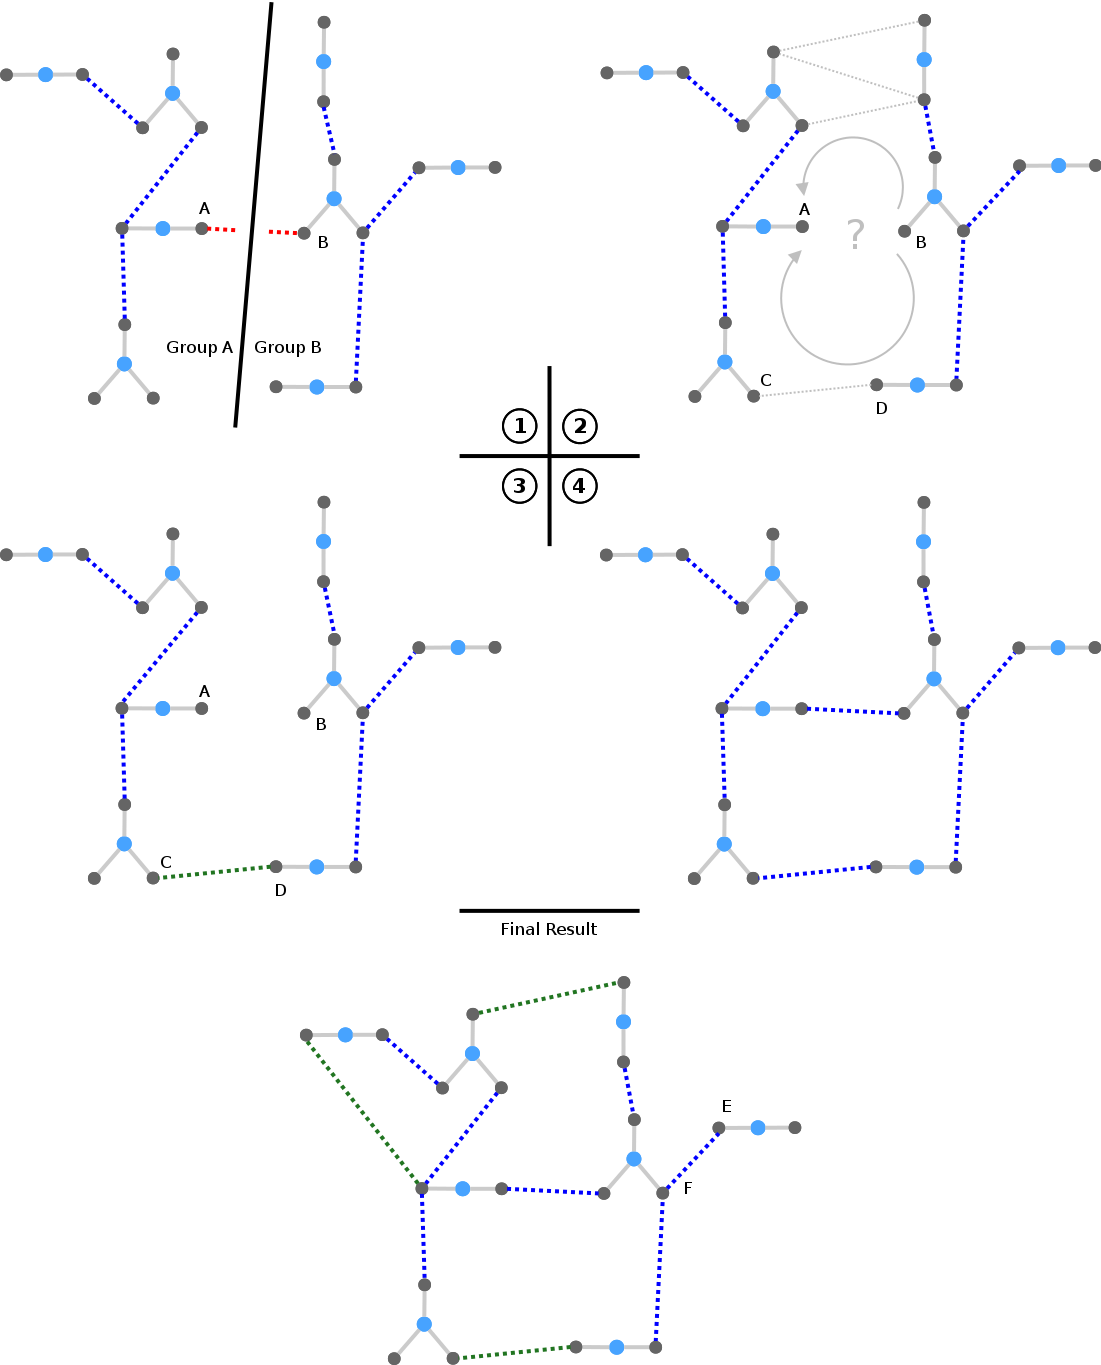
\includegraphics[width=1\columnwidth]{figures/survival_algo2}
      \caption{Finding survival paths. Simulation of connection between node A and node B failing, creating two groups.
	Finding a survival path for node A and B. Eventually all connections have a survival path. No redundant link possible for failing connection (E, F).}
      \label{fig:survival_algo}
    \end{figure}
    
    \begin{table}[h!]
      \centering
      \begin{tabular}{|c|c|}\hline
	Channel & Interference Count\\ \hline
	36 & 4 \\ \hline
	\textbf{11} & \textbf{1} \\ \hline
	\textbf{1} & \textbf{1} \\ \hline
      \end{tabular}
      \begin{tabular}{|c|c|}\hline
	Channel & Interference Count\\ \hline
	\textbf{36} & \textbf{4} \\ \hline
	11 & 5 \\ \hline
	1 & 5  \\ \hline
      \end{tabular}
      \caption{Channel-list without (left) and with (right) foreign influence}
    \end{table}
    
\newpage
    
  \section{Channel Assignment Algorithm}
    For a given network topology graph and a set of channels to chose from, we can now assign channels to the module-nodes or if you like the links
    between those. Therefore we iterate over all module-module edges and assign channels to the adjacent module-nodes if they do not already have one assigned.
    The channel for an edge is chosen by the following pattern for each channel-group:
    Select all the modules which are connected by module-module edges. This set of nodes is called the channel-group.
    For this channel group we create a list of channels and corresponding interference occurrences.
    Among these we pick those channels from the set of all possible channels, which have been used the least in this channel-list. If there is a tie in usage
    we can additionally respect foreign networks by taking the occurrences of foreign radio modules also into account. Since we do not know how much traffic the foreign 
    channels carry and therefore how much they utilize the channels, we can only weight them equally compared to our own channel-usage instead of a more fine-grained subdivision.
    As a further tie-breaker we pick those channels which have been used the least in general.
    At last we resort to just selecting one channel at random, but this should rarely occur.
    Especially respecting foreign networks allows use to evade heavily used bands and channels like for example 1 and 11 in the 2.4 GHz band which 
    are used by devices out of our control.
    
    \begin{figure}[h!]
      \centering
      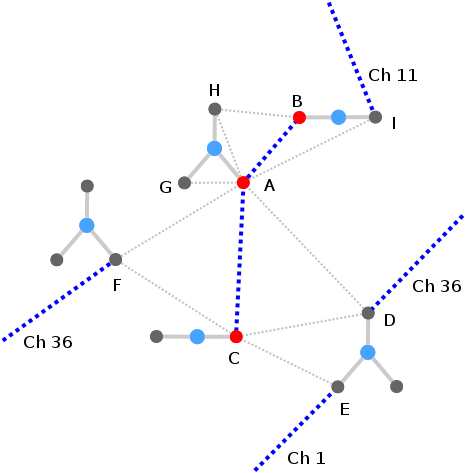
\includegraphics[width=0.7\columnwidth]{figures/channel-list}
      \caption{Channelset A,B,C selected for coloring.}
      \label{fig:channel-list}
    \end{figure}
    
\newpage
    
    Since A, B and C are in the receive range of D, E, F, G, H, I they are possible sources of interference if we use the same channel as those. 
    Therefore we survey how often every channel interferes, where one module can also interfere multiple times.
    For example does module F which already has channel 36 assigned interfere 4 times with the channel-set A,B,C ((A, F), (C, F), (C, D), (A, D)). 
    If we only could choose from channel 1,11 and 36 we would then decide to use
    channel 1 or 11 to assign to the channel-set depending on how often we overall used those already.
    If however we want to take also foreign networks into consideration and lets say modules A and C would both detect two other \ac{WLAN} networks at channel 11 and two
    at channel 1, then we would add another 4 for channel 11 and channel 1 in the channel-list, leading to Channel 36 as the best choice. 
    Note modules G and H are ignored for the counting process since they do not have links or channels assigned.
    
    \begin{figure}[h!]
      \centering
      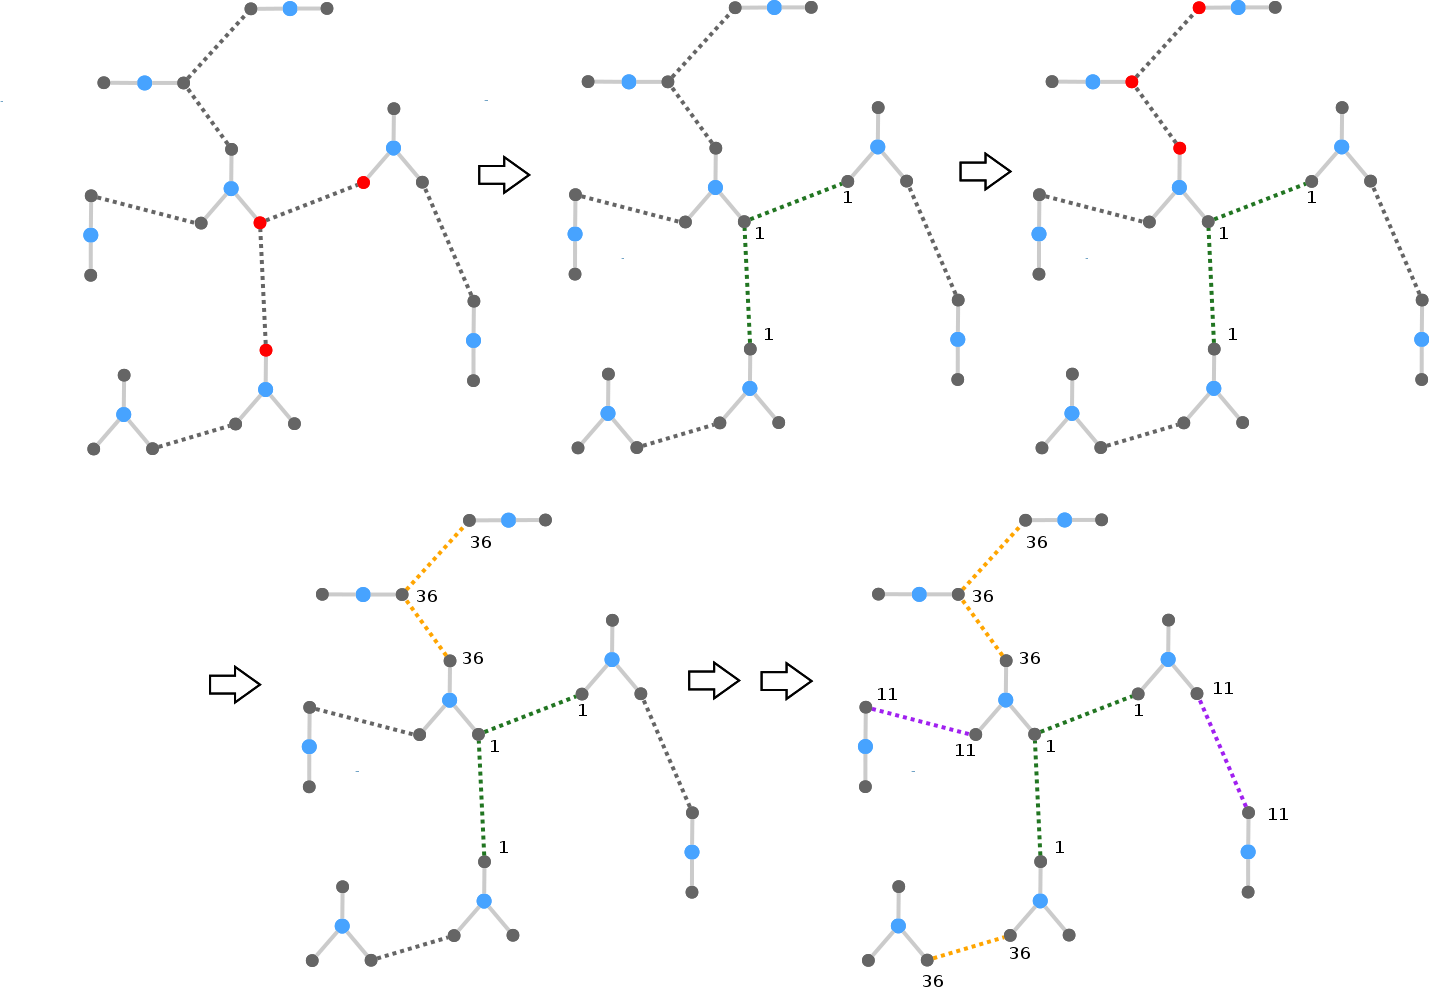
\includegraphics[width=1\columnwidth]{figures/caa_algo}
      \caption{General overview on the channel assignment process.}
      \label{fig:caa_algo}
    \end{figure}

    Figure \ref{fig:caa_algo} shows an example-assignment for a network with 8 APs with 2 and 3 modules equipped and available channels [1, 11, 36] without foreign influence. 
    Each graph depicts the status after each of the assingments. 
    Red marked nodes represent a channel-group. 
    Currently there is no special order in which the channel-sets are colored. 
